\documentclass[../main/main.tex]{subfiles}

% \toggletrue{student}
% \HideSolutionstrue

\raggedbottom

\makeatletter
\renewcommand{\@chapapp}{Induction -- chapitre}
\makeatother

\begin{document}
\setcounter{chapter}{3}
\chapter{Conversion électromécanique}
\label{ch:convelecmeca}

On a vu précédemment quelques exemples où un mouvement mécanique créé un champ
électrique, mais également l'inverse. Un peu de vocabulaire~:
\begin{itemize}[label=$\diamond$, leftmargin=10pt]
  \item On parle de circuit \textbf{moteur} lorsqu'il convertit une puissance
    de \textbf{électrique à mécanique}~;
  \item On parle de circuit \textbf{générateur} lorsqu'il convertit une puissance
    de \textbf{mécanique à électrique}.
\end{itemize}
\begin{figure}[h]
  \centering
  \switch{
    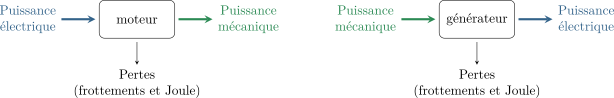
\includegraphics[scale=1]{motgene}
  }{
    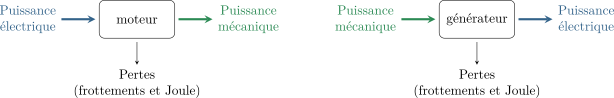
\includegraphics[scale=1, draft=true]{motgene}
  }
  \caption{Schématisation des fonctionnements moteur et générateur.}
  \label{fig:motgene}
\end{figure}
\vspace*{-20pt}

\section{Conversion de puissance électrique en puissance mécanique}
\label{sec:convelecmeca}
\subsection{Exemple des rails de \textsc{Laplace} moteurs}
\label{ssec:rlplmot}
\begin{tdefi}{Définition, hand}
  \cswitch{white}{
    Les rails de \textsc{Laplace} \textbf{moteurs} sont deux conducteurs
    rectilignes parallèles reliés par une tige mobile conductrice rendant le
    circuit \textbf{déformable}, plongé dans un champ magnétique constant
    perpendiculaire au circuit et \textbf{alimenté par une f.é.m.\ constante
    $U_0$}.
  }
\end{tdefi}
Le générateur étant dans un circuit fermé, il impose un courant $i > 0$.
\textbf{On néglige l'auto-induction}, et on appelle $R$ la résistance totale du
circuit. Nous avons déjà constaté expérimentalement la mise en mouvement de la
barre à l'aide de la force de \textsc{Laplace}. Quelle vitesse atteint-elle~?
\begin{figure}[h]
  \centering
  \switch{
    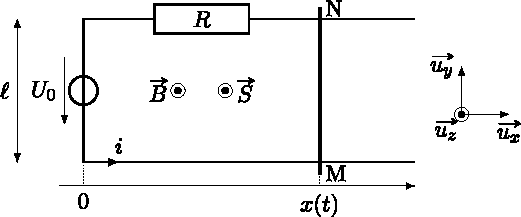
\includegraphics[scale=1]{rlplmot_schema}
  }{
    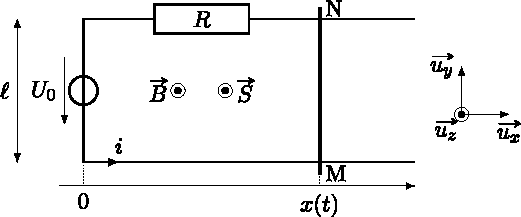
\includegraphics[scale=1, draft=true]{rlplmot_schema}
  }
  \caption{Rails de \textsc{Laplace} moteurs.}
  \label{fig:rlplmot_schema}
\end{figure}
\vspace*{-20pt}

\subsubsection{Analyse qualitative}
\label{ssec:rlplmot_anaqual}
\begin{figure}[h]
  \centering
  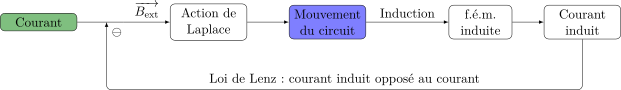
\includegraphics[scale=1]{modlenz_rlplmot}
  \caption{Schéma de causalité des conséquences de l'induction.}
  \label{fig:modlenz_rlplmot}
\end{figure}
Avant de se lancer dans les calculs, on peut déterminer le comportement du
système avec la loi de \textsc{Lenz}. À l'origine de l'induction est la présence
d'un champ extérieur $\vv{B_{\rm ext}}$ et d'un courant dans le circuit.
Combinés ensemble, ils appliquent une action de \textsc{Laplace} sur le barreau,
le mettant en mouvement et \textbf{déformant} le circuit. Il y a donc
\textbf{variation du flux}, et d'après la loi de \textsc{Faraday} une f.é.m.\
induite y apparaît. Le circuit étant toujours fermé, il y a également un courant
induit.
\smallbreak
L'induction modérant, par ses conséquences, les causes qui lui ont donné
naissance, on en conclut que ce \textbf{courant induit s'oppose au courant
initial}, ce qui générera une force de \textsc{Laplace} opposée tendant à
freiner l'accélération du barreau. On veut étudier ce comportement et notamment
connaître la vitesse finale~: est-elle infinie~? nulle~? constante~?

\begin{timpo}{Attention, hand}
  \begin{center}
    \danger\
    \cswitch{white}{
      Une étude de causalité doit comparer une conséquence et une cause de
      mêmes natures~!
    }
    \danger
  \end{center}
\end{timpo}

\subsubsection{Analyse mécanique}
\label{sssec:rlplmot_anameca}
On étudie le mouvement de la barre de masse $m$ dans le référentiel de la
salle de classe. Avec un bilan des forces~:
\begin{itemize}[label=$\diamond$, leftmargin=10pt]
  \litem{\cswitch{white}{Poids}} \cswitch{white}{
    $\vv{P} = m \vv{g} = -mg\uz$~;
  }
  \litem{\cswitch{white}{Réaction normale}} \cswitch{white}{
    $\vv{N} = N\uz$~;
  }
  \litem{\cswitch{white}{Force de \textsc{Laplace}}} \cswitch{white}{
    $\vv{F_{\rm Lap}} = i \vv{\rm MN}\wedge \vv{B} = i \ell B \ux$~;
  }
  \litem{\cswitch{white}{Frottements}} \cswitch{white}{
    $\vv{F_f} = -F_f \ux$ avec $F_f > 0$.
  }
\end{itemize}
Ainsi,
\cswitch{white}{
  \[
    m \dv{\vv{v}}{t} = \vv{P} + \vv{F_{\rm Lap}} + \vv{N} + \vv{F_f}
  \]
}
D'où, en projetant sur $\ux$~:
\begin{tprop}{Équation mécanique, hand}
  \cswitch{white}{
    \begin{equation}
      \usetagform{black}
      \label{eq:eqmeca}
      m \dv{v}{t} = i \ell B - F_f
    \end{equation}
    \vspace*{-10pt}
  }
\end{tprop}

\subsubsection{Analyse électrique}
\label{sssec:rlplmot_anaelec}
La déformation du circuit entraîne une variation de sa surface. Ainsi, même avec
un champ magnétique constant, le flux magnétique varie, impliquant l'apparition
d'une f.é.m.\ induite.
\bigbreak
\noindent
Avec $\vv{S} = S\uz$ pris dans le sens de $i$, on trouve pour $\F$~:
\cswitch{white}{
  \[
    \F = B\uz \cdot S\uz = BS = B \ell x
  \]
}
D'où, avec la loi de \textsc{Faraday}~:
\cswitch{white}{
  \[
    e = -\dv{\F}{t} = -B \ell \dot{x}
  \]
}
Placée en \textbf{convention générateur}. Donc, avec la loi des mailles~:
\cswitch{white}{
  \[
    e+U_0 = Ri \quad \Ra \quad U_0 = Ri + B \ell \dot{x}
  \]
}
Ainsi,
\begin{tprop}{Équation électrique, hand}
  \cswitch{white}{
    \begin{equation}
      \usetagform{black}
      \label{eq:eqelec}
      U_0 = Ri + B \ell v
    \end{equation}
    \vspace*{-10pt}
  }
\end{tprop}

\subsubsection{Résolution}
\label{sssec:rlplmot_resol}
On cherche à éliminer $i$ pour obtenir une équation différentielle sur $v$. On
l'isole dans \eqref{eq:eqelec}~:
\cswitch{white}{
  \[
    i = \frac{U_0}{R} - \frac{B \ell }{R}v
  \]
}
Et on substitue $i$ dans l'équation mécanique \eqref{eq:eqmeca} \textbf{en
l'absence de frottements}~:
\cswitch{white}{
  \begin{align*}
    m \dv{v}{t} &= \left( \frac{U_0}{R} - \frac{B \ell }{R} \right) \ell B
    \\\Lra 
    m \dv{v}{t} &= \frac{U_0 \ell B}{R} - \frac{B^2 \ell ^{2}}{R}v
    \\\Lra 
    \Aboxed{\dv{v}{t} + \frac{B^2 \ell ^{2}}{Rm}v &= \frac{U_0 \ell B}{Rm}}
  \end{align*}
}
On obtient donc une équation différentielle de la forme~:
\cswitch{white}{
  \[
    \boxed{\dv{v}{t} + \frac{v}{\tau} = \frac{v_{\rm lim}}{\tau}}
    \qav
    \boxed{\tau = \frac{Rm}{B^2 \ell ^{2}}}
    \qet
    \boxed{v_{\rm lim} = \frac{U_0}{B \ell }}
  \]
}
Qui se résout en
\cswitch{white}{
  \[
    \boxed{v(t) = v_{\rm lim}\left( 1 - \exr^{-t/\tau} \right)}
    \Lra 
    \boxed{i(t) = \frac{U_0}{R}\exr^{-t/\tau}}
  \]
}
Ainsi, l'\textbf{intensité finit par être nulle} et \textbf{la vitesse du rail
finit par atteindre une valeur limite}.

\subsubsection{Résumé méthode}
\label{sssec:rlplmot_mth}
\begin{tror}{Méthode, heart}
  \begin{enumerate}
    \item \cswitch{white}{
      Obtenir l'équation mécanique~:
    }
    \begin{itemize}[label=$\diamond$, leftmargin=20pt]
      \item \cswitch{white}{
        PFD si translation
      }
      \item \cswitch{white}{
        TMC si rotation
      }
    \end{itemize}
    \item \cswitch{white}{
      Obtenir l'équation électrique~:
    }
    \begin{enumerate}
      \item \cswitch{white}{
        Définir un sens pour le courant, avoir $\vv{S}$, calculer $\F$~;
      }
      \item \cswitch{white}{
        Utiliser la loi de \textsc{Faraday} pour avoir la f.é.m.\ induite~;
      }
      \item \cswitch{white}{
        L'ajouter dans le circuit en \textbf{convention générateur}~;
      }
      \item \cswitch{white}{
        Appliquer la loi des mailles
      }
    \end{enumerate}
    \item \cswitch{white}{
      Résoudre les équations couplées
    }
  \end{enumerate}
\end{tror}

\subsubsection{Bilan énergétique}
\label{sssec:rlplmot_bilanrj}
\begin{itemize}[label=$\diamond$, leftmargin=10pt]
  \litem{Bilan électrique}~: \cswitch{white}{
    On multiplie la LdM par $i$~:
    \[
      U_0i = Ri^2 + B \ell vi
    \]
  } On identifie~:
  \begin{itemize}[label=$\triangleright$, leftmargin=20pt]
    \item puissance du générateur~: \cswitch{white}{
      $\mathcal{P}_g = U_0i$
    }
    \item puissance dissipée par effet Joule~: \cswitch{white}{
      $\mathcal{P}_J = Ri^2$
    }
    \item puissance reçue par la f.é.m.~: \cswitch{white}{
      $\mathcal{P}_e = -ei = B \ell vi$
    }
  \end{itemize}
  Ainsi,
  \cswitch{white}{
    \[
      \boxed{\mathcal{P}_g = \mathcal{P}_J + \mathcal{P}_e}
    \]
  }
  \litem{Bilan mécanique}~: \cswitch{white}{
    On multiplie le PFD par $v$~:
    \[
      mv \dv{v}{t} = i \ell Bv - F_f v
    \]
  } On identifie~:
  \begin{itemize}[label=$\triangleright$, leftmargin=20pt]
    \item dérivée de l'énergie cinétique~: \cswitch{white}{
      $\dv{\mathcal{E}_c}{t} = mv \dv{v}{t}$
    }
    \item puissance des forces de \textsc{Laplace}~: \cswitch{white}{
      $\mathcal{P}_{\rm Lap} = i \ell Bv$
    }
    \item puissance perdue par frottements~: \cswitch{white}{
      $\mathcal{P}_f = -(-F_fv) = F_fv$
    }
  \end{itemize}
  Ainsi,
  \cswitch{white}{
    \[
      \boxed{\dv{\mathcal{E}_c}{t} + \mathcal{P}_f = \mathcal{P}_{\rm Lap}}
    \]
  }
\end{itemize}
On remarque notamment que
\[
  \mathcal{P}_e = \mathcal{P}_{\rm Lap}
\]
C'est-à-dire que le \textbf{couplage électromécanique est parfait}~: la
puissance électrique reçue par la force électromotrice induite est égale à la
puissance mécanique (motrice) des forces de \textsc{Laplace}. Ainsi, en
définissant le rendement par
\[
  \boxed{\eta = \abs{\frac{\text{puissance utile}}{\text{puissance fournie}}}}
\]
on voit que \textbf{contrairement à la thermodynamique}, le \textbf{rendement
théorique} de conversion électromécanique est de 1~! En effet, seules les
\textbf{pertes limitent le transfert}.

\subsubsection{Bilan global}
\label{sssec:rlplmot_bilanglb}
En combinant les résultats de puissance, on a mathématiquement puis
schématiquement~:
\[
  \boxed{\Pc_g = \Pc_J + \Pc_f + \dv{\Ec_c}{t}}
\]
\begin{figure}[h!]
  \centering
  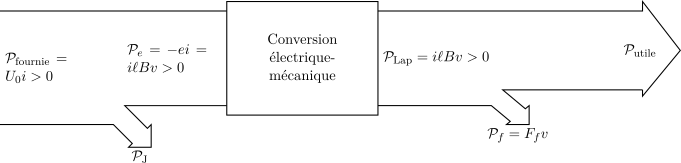
\includegraphics[scale=1]{rlplmot_bilan}
  \label{fig:rlplmot_bilan}
\end{figure}

\newpage

\subsection{Le moteur à entrefer plan}
\label{ssec:motentrefer}


\end{document}
